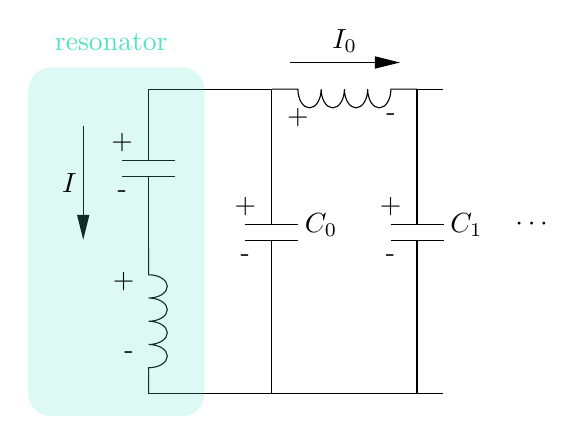
\begin{tikzpicture}[x=0.75pt,y=0.75pt,yscale=-1,xscale=1]
    %uncomment if require: \path (0,322); %set diagram left start at 0, and has height of 322
    
    %Straight Lines [id:da11749834712937979] 
    \draw    (339.83,276.15) -- (409.83,276.15) ;
    %Shape: Capacitor [id:dp09598906024538234] 
    \draw   (339.83,160.04) -- (339.83,194.61) (352.58,202.29) -- (327.08,202.29) (352.58,194.61) -- (327.08,194.61) (339.83,202.29) -- (339.83,236.85) ;
    %Shape: Inductor (Air Core) [id:dp8899610885698173] 
    \draw   (409.83,129.33) -- (397.23,129.33) .. controls (397.23,134.3) and (394.72,138.33) .. (391.63,138.33) .. controls (388.54,138.33) and (386.03,134.3) .. (386.03,129.33) .. controls (386.03,134.3) and (383.52,138.33) .. (380.43,138.33) .. controls (377.34,138.33) and (374.83,134.3) .. (374.83,129.33) .. controls (374.83,134.3) and (372.32,138.33) .. (369.23,138.33) .. controls (366.14,138.33) and (363.63,134.3) .. (363.63,129.33) .. controls (363.63,134.3) and (361.12,138.33) .. (358.03,138.33) .. controls (354.94,138.33) and (352.43,134.3) .. (352.43,129.33) -- (339.83,129.33) ;
    %Straight Lines [id:da4427013233239925] 
    \draw    (409.83,129.33) -- (422.33,129.33) ;
    %Straight Lines [id:da8544967510982182] 
    \draw    (280.5,276.15) -- (339.83,276.15) ;
    %Straight Lines [id:da3980805643302381] 
    \draw    (409.83,276.15) -- (422.33,276.15) ;
    %Straight Lines [id:da021438736433621264] 
    \draw    (280.5,129.33) -- (339.83,129.33) ;
    %Shape: Capacitor [id:dp20286796618144542] 
    \draw   (280.5,129.33) -- (280.5,163.9) (293.25,171.58) -- (267.75,171.58) (293.25,163.9) -- (267.75,163.9) (280.5,171.58) -- (280.5,206.15) ;
    %Shape: Inductor (Air Core) [id:dp461246695780545] 
    \draw   (280.5,206.15) -- (280.5,218.75) .. controls (285.47,218.75) and (289.5,221.26) .. (289.5,224.35) .. controls (289.5,227.44) and (285.47,229.95) .. (280.5,229.95) .. controls (285.47,229.95) and (289.5,232.46) .. (289.5,235.55) .. controls (289.5,238.64) and (285.47,241.15) .. (280.5,241.15) .. controls (285.47,241.15) and (289.5,243.66) .. (289.5,246.75) .. controls (289.5,249.84) and (285.47,252.35) .. (280.5,252.35) .. controls (285.47,252.35) and (289.5,254.86) .. (289.5,257.95) .. controls (289.5,261.04) and (285.47,263.55) .. (280.5,263.55) -- (280.5,276.15) ;
    %Straight Lines [id:da3713429559344812] 
    \draw    (339.83,236.85) -- (339.83,276.15) ;
    %Straight Lines [id:da19554953394992203] 
    \draw    (339.83,129.33) -- (339.83,160.04) ;
    %Shape: Capacitor [id:dp008034011040416456] 
    \draw   (409.83,160.04) -- (409.83,194.61) (422.58,202.29) -- (397.08,202.29) (422.58,194.61) -- (397.08,194.61) (409.83,202.29) -- (409.83,236.85) ;
    %Straight Lines [id:da07456917566674814] 
    \draw    (409.83,236.85) -- (409.83,276.15) ;
    %Straight Lines [id:da1286310190144886] 
    \draw    (409.83,129.33) -- (409.83,160.04) ;
    %Straight Lines [id:da6895241562197532] 
    \draw    (249,147) -- (249,199.85) ;
    \draw [shift={(249,201.85)}, rotate = 270] [fill={rgb, 255:red, 0; green, 0; blue, 0 }  ][line width=0.08]  [draw opacity=0] (12,-3) -- (0,0) -- (12,3) -- cycle    ;
    %Straight Lines [id:da6652369709419201] 
    \draw    (348.43,116.48) -- (399.5,116.48) ;
    \draw [shift={(401.5,116.48)}, rotate = 180] [fill={rgb, 255:red, 0; green, 0; blue, 0 }  ][line width=0.08]  [draw opacity=0] (12,-3) -- (0,0) -- (12,3) -- cycle    ;
    %Rounded Rect [id:dp3218082028954583] 
    \draw  [draw opacity=0][fill={rgb, 255:red, 80; green, 227; blue, 194 }  ,fill opacity=0.2 ] (222.5,129.85) .. controls (222.5,123.78) and (227.42,118.85) .. (233.5,118.85) -- (296.5,118.85) .. controls (302.58,118.85) and (307.5,123.78) .. (307.5,129.85) -- (307.5,275.85) .. controls (307.5,281.93) and (302.58,286.85) .. (296.5,286.85) -- (233.5,286.85) .. controls (227.42,286.85) and (222.5,281.93) .. (222.5,275.85) -- cycle ;
    
    % Text Node
    \draw (456,190.4) node [anchor=north west][inner sep=0.75pt]    {$\cdots $};
    % Text Node
    \draw (327.08,191.61) node [anchor=south] [inner sep=0.75pt]   [align=left] {+};
    % Text Node
    \draw (327.08,205.29) node [anchor=north] [inner sep=0.75pt]   [align=left] {\mbox{-}};
    % Text Node
    \draw (267.75,160.9) node [anchor=south] [inner sep=0.75pt]   [align=left] {+};
    % Text Node
    \draw (268.5,227.75) node [anchor=south] [inner sep=0.75pt]   [align=left] {+};
    % Text Node
    \draw (267.75,174.58) node [anchor=north] [inner sep=0.75pt]   [align=left] {\mbox{-}};
    % Text Node
    \draw (271.08,252.29) node [anchor=north] [inner sep=0.75pt]   [align=left] {\mbox{-}};
    % Text Node
    \draw (247,174.43) node [anchor=east] [inner sep=0.75pt]    {$I$};
    % Text Node
    \draw (374.97,113.08) node [anchor=south] [inner sep=0.75pt]    {$I_{0}$};
    % Text Node
    \draw (354.58,194.61) node [anchor=west] [inner sep=0.75pt]    {$C_{0}$};
    % Text Node
    \draw (424.58,194.61) node [anchor=west] [inner sep=0.75pt]    {$C_{1}$};
    % Text Node
    \draw (397.08,191.61) node [anchor=south] [inner sep=0.75pt]   [align=left] {+};
    % Text Node
    \draw (397.08,205.29) node [anchor=north] [inner sep=0.75pt]   [align=left] {\mbox{-}};
    % Text Node
    \draw (352.43,137.33) node [anchor=north] [inner sep=0.75pt]   [align=left] {+};
    % Text Node
    \draw (397.23,137.33) node [anchor=north] [inner sep=0.75pt]   [align=left] {\mbox{-}};
    % Text Node
    \draw (262.47,111.85) node [anchor=south] [inner sep=0.75pt]  [color={rgb, 255:red, 80; green, 227; blue, 194 }  ,opacity=1 ] [align=left] {resonator};
    
    
    \end{tikzpicture}
    